% !TEX program = lualatex
% !BIB program = biber

% ==============================================================================
% Tutorial: Animation
% ==============================================================================
% \pause: for generally reveal items
% \item<1->\n \item<2->: similar to pause, display items one by one. 
% \only<1>{content}: only show content in slide no. 1. For replacing items in next slide. 

% ==============================================================================
% Tutorial: Fonts
% ==============================================================================
% math font: 
% 	\usefonttheme[onlymath]{serif}: use serif style math font

% ==============================================================================
% Tutorial: Block environment
% ==============================================================================
% Three blocks: 
% 	block
% 	alertblock
% 	exampleblock
% \begin{block}{title}
% 	content
% \end{block}
% \metroset{block=fill}: use background color, if not, the background is white. 

% ==============================================================================
% Tutorial: Sign and symbols
% ==============================================================================
% \setbeamertemplate{section in toc}[square]: set symbols in front of a section in table of content. 

\documentclass[8pt,dvipsnames,table]{beamer}

% ==============================================================================
% Language and Encoding
% ==============================================================================
\usepackage[utf8]{inputenc}
\usepackage[american]{babel}
% \usepackage[square,sort]{natbib}
\usepackage[backend=biber,style=apa]{biblatex}

% ==============================================================================
% BibLaTeX configuration
% ==============================================================================
\addbibresource{../Bib.bib}
\DeclareLanguageMapping{american}{american-apa}

% ==============================================================================
% Font
% ==============================================================================
% \usefonttheme{professionalfonts}
% \usefonttheme{serif}
% \usepackage[T1]{fontspec}
% \setmainfont{Helvetica Neue}
\usepackage[scaled]{helvet}
\usepackage{lmodern}
% \usepackage{fourier}
% \usepackage{kmath}
% \usepackage[OT1]{eulervm}
\usefonttheme[onlymath]{serif}

% ==============================================================================
% Color, style and layout
% ==============================================================================
\usepackage{xcolor}
\usepackage{graphicx}
\usepackage{hyperref}
\usepackage{bm}
\usepackage{subfig}
\usepackage{pict2e}
\usepackage{comment}
\usepackage{pdfpages}
\usepackage{geometry}
% \usepackage[paper=landscape]{typearea}

% ==============================================================================
% Math and Physics
% ==============================================================================
\usepackage{mathrsfs}
\usepackage{physics}
\usepackage{slashed}
\usepackage{siunitx}
\usepackage{tikz-feynman}
\usepackage{extarrows}

% ==============================================================================
% Beamer backup
% ==============================================================================
\usepackage{appendixnumberbeamer}

% ==============================================================================
% Theme
% ==============================================================================
\usetheme{metropolis}
% \usecolortheme[snowy]{owl}
\linespread{1.5}

% ==============================================================================
% Macros
% ==============================================================================
%\newcommand{\phanitem}{\phantom{\item}}
\newcommand{\lag}{\mathcal{L}}
\newcommand{\Mcal}{\mathcal{M}}
\newcommand{\g}{\gamma}
\renewcommand{\a}{\alpha}
\newcommand{\s}{\sigma}
\newcommand{\calA}{\mathcal{A}}
\newcommand{\mm}[1]{\frac{\dd^4#1}{(2\pi)^4}}
\newcommand{\mme}[1]{\frac{\dd^3\vb{#1}}{(2\pi)^3}}
\newcommand{\mmd}[2][d]{\frac{\dd^{#1}{#2}}{(2\pi)^{#1}}}

% ==============================================================================
% Color Command
% ==============================================================================
% \definecolor{red}{rgb}{1, 0., 0.}

\newcommand{\red}[1]{{\color{OrangeRed}#1}}
\newcommand{\orange}[1]{{\color{Bittersweet}#1}}
\newcommand{\blue}[1]{{\color{NavyBlue}#1}}
\newcommand{\green}[1]{{\color{ForestGreen}#1}}
\newcommand{\purple}[1]{{\color{RedViolet}#1}}

% ==============================================================================
% Itemize style
% ==============================================================================
\setbeamertemplate{itemize item}{$\square$}

% ==============================================================================
% Horizontal Alignment
% ==============================================================================
\makeatletter
\newcommand{\pushright}[1]{\ifmeasuring@#1\else\omit\hfill$\displaystyle#1$\fi\ignorespaces}
\newcommand{\pushleft}[1]{\ifmeasuring@#1\else\omit$\displaystyle#1$\hfill\fi\ignorespaces}
\makeatother

% ==============================================================================
% Graphics Path
% ==============================================================================
\graphicspath{./}

% ==============================================================================
% Tikz Externalization
% ==============================================================================
% \usepackage{shellesc}
% \usetikzlibrary{external}
% % \usepgfplotslibrary{external}
% \tikzexternalize[shell escape=-enable-write18,prefix=./,system call={lualatex \tikzexternalcheckshellescape -halt-on-error -interaction=batchmode -jobname "\image" "\texsource"},up to date check=md5]


% ==============================================================================
% Title Page
% ==============================================================================
\title{Tan Relations within QFT Framework}
\author[Y. Huang]{Yingsheng Huang}
\institute[IHEP]{Institute of High Energy Physics}
\date

\metroset{block=fill}
\setbeamertemplate{section in toc}[square]

\begin{document}

\begin{frame}{}
	\maketitle
	% \par\medskip
	% \uncover<4->{\vsapce*{-3in}arxiv:1809.09023}
\end{frame}

\begin{frame}
	\frametitle{Outlines}
	\tableofcontents
\end{frame}


\section{What're Tan Relations?}
\begin{frame}
	\frametitle{Ultracold Atomic Fermi Gas}

	\begin{itemize}
		\item dilute gases
		\item only has short range interaction
		\item when scattering length is much larger than the range of the force, short range details become insignificant, we can mimic the effect with a delta potential
		\item within a small range of scattering length $a$, similar to nuclear system
	\end{itemize}


\end{frame}
\begin{frame}
	\frametitle{Tan Relations}

	A set of relations representing physical quantities with a universal function $C$, the \emph{integrated contact density} or simply \emph{contact}, in large momentum limit~\parencite{Tan2008,Tan2008a,Tan_2008}.
	\begin{alertblock}{Contact}
		$$C\equiv\int\dd^3R\expval{g^2\psi^\dagger_1\psi^\dagger_2\psi_1\psi_2(R)}$$
	\end{alertblock}

	\only<1>{
		\begin{block}{Energy relation}
			$$E = \sum_{\sigma} \int \frac {d^{3} k} {(2 \pi)^{3}} \frac {k^{2}} {2 m} \left(\rho_{\sigma} (k) - \frac {C} {k^{4}}\right) + \frac {C} {4 \pi m a}+ \int d^{3} R \langle V \rangle$$
		\end{block}
		\begin{block}{Adiabatic relation}
			$$\frac {\dd E} {\dd (1 / a)} = - \frac {1} {4 \pi m} C$$
		\end{block}
	}

	\only<2>{
		\begin{block}{Virial theorem}
			$$E=2 \int d^{3} R\langle\mathcal{V}\rangle-C /(8 \pi m a)$$
		\end{block}
		\begin{block}{Momentum distribution}
			$$\rho_{\sigma}(\boldsymbol{k}) \longrightarrow C / k^{4}$$
		\end{block}
		\begin{block}{Number density of fermion pairs}
			$$\left\langle N_{\text {pair }}(\boldsymbol{R}, \boldsymbol{s})\right\rangle \longrightarrow s^1$$
		\end{block}
	}
\end{frame}

\section{Pionless EFT}

\begin{frame}
	\frametitle{Pionless EFT}

	\begin{itemize}
		\item Successful in describing nuclei. \setlength{\itemsep}{20mm}
		\item Introduced for few body atomic systems~\parencite[see review by][]{Platter2009}.
		
		The use of contact interaction in an EFT for dilute gases can be dated to the '90s.
	\end{itemize}

\end{frame}

\begin{frame}
	\frametitle{Effective Range Expansion}

	At zero energy limit
	\begin{align*}
		u(r\gg R)\approx 1-r/a
	\end{align*}

	\begin{block}{ERE}
		\begin{align}
			k \cot \delta_{0}=-\frac{1}{a}+\frac{r_{s}}{2} k^{2}+\cdots
		\end{align}
	\end{block}
	The amplitude is
	\begin{align}
		\begin{aligned}
			T & =\frac{4 \pi}{m} \frac{1}{k \cot \delta-i k}                                   \\
			  & =\frac{4 \pi}{m} \frac{1}{-\frac{1}{a_{s}}+\frac{r_{0s} }{2} k^{2}+\ldots-i k}
		\end{aligned}
	\end{align}

\end{frame}

\begin{frame}
	\frametitle{Lagrangian~\parencite{Bedaque2002}}

	\begin{alertblock}{Pionless EFT Lagrangian}
		\begin{align}
			\begin{aligned}
				\mathcal{L}_{\mathrm{eft}} & =\psi^{\dagger}\left[i \frac{\partial}{\partial t}+\frac{\vec{\nabla}^{2}}{2 m}\right] \psi-\frac{C_{0}}{2}\left(\psi^{\dagger} \psi\right)^{2}+\frac{C_{2}}{16}\left[(\psi \psi)^{\dagger}\left(\psi \stackrel{\leftrightarrow}{\nabla}^{2} \psi\right)+\mathrm{h.c.}\right] \\
				                           & +\frac{C_{2}^{\prime}}{8}(\psi \vec{\nabla} \psi)^{\dagger} \cdot(\psi \vec{\nabla} \psi)-\frac{D_{0}}{6}\left(\psi^{\dagger} \psi\right)^{3}+\ldots
			\end{aligned}
		\end{align}
	\end{alertblock}
	We only consider the leading order, which contains only $C_0$ term. This leaves us (using a dimensionless coupling constant $g(\Lambda)$)
	\begin{alertblock}{Leading order Pionless EFT Lagrangian}
		\begin{align}
			\mathcal{L} & =\psi^{\dagger}\left[i \frac{\partial}{\partial t}+\frac{\vec{\nabla}^{2}}{2 m}\right] \psi-\frac{g(\Lambda)}{m}\left(\psi^{\dagger} \psi\right)^{2}
		\end{align}
	\end{alertblock}
	There's no gauge symmetry present. However, one could introduce new fields and currents that has gauge symmetry, i.e. include photons to account for isospin breaking effect. So far these're all fixed by NN scattering data, there're also terms need extra data.

\end{frame}

\begin{frame}
	\frametitle{Bubble resum}

	Consider:
	\begin{align}
		i\calA=\mel{34}{\psi^\dagger\psi}{12}=
		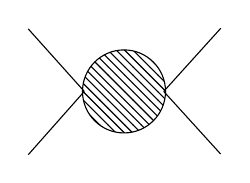
\begin{tikzpicture}[baseline=(o1.base)]
			\begin{feynman}
				\diagram[small,horizontal=o1 to o3]{
				p1 -- o1 --[draw=none] o3 -- p3;
				p2 -- o1 --[draw=none] o3 -- p4;
				};
				\node[blob, minimum size=30pt] at ($(o1)!0.5!(o3)$) (o2);
			\end{feynman}
		\end{tikzpicture}
	\end{align}
	Define $P=p_1+p_2=(E,\vb{0})$, and $E=p^2/m$.
	The integral equation is
	\begin{align}
		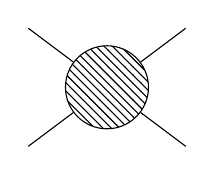
\begin{tikzpicture}[baseline=(o1.base)]
			\begin{feynman}
				\diagram[small,horizontal=p1 to p3,layered layout]{
					p1 -- o1[blob, minimum size=30pt] -- p3;
					p2 -- o1 -- p4;
					{[same layer]p1,p2};
				};
				% \node[blob, minimum size=30pt] at (o1);
			\end{feynman}
		\end{tikzpicture}=
		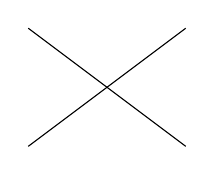
\begin{tikzpicture}[baseline=(o3.base)]
			\begin{feynman}
				\diagram[small,layered layout,horizontal=p1 to p3]{
					p1 -- o3 -- p3;
					p2 -- o3 -- p4;
				};
				\node at (o3);
			\end{feynman}
		\end{tikzpicture}+
		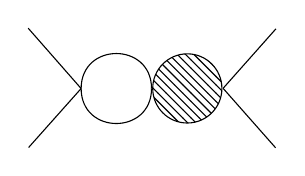
\begin{tikzpicture}[baseline=(o3.base)]
			\begin{feynman}
				\diagram[small,horizontal=o3 to o4]{
				p1 -- o3 --[draw=none] o4 --[draw=none] o6 -- p3;
				p2 -- o3 --[draw=none] o4 --[draw=none] o6 -- p4;
				};
				\diagram*{
				(o3) --[half left,looseness=1.7] (o4);
				(o3) --[half right,looseness=1.7] (o4);
				};
				\node[blob, minimum size=25pt] at ($(o4)!0.5!(o6)$) (o5);
			\end{feynman}
		\end{tikzpicture}
	\end{align}

	\begin{align}
		i\calA=-\frac{ig(\Lambda)}{m}\pqty{1+i\calA\int\mm{k}\frac{i}{k^0-\frac{\vb{k}^2}{2m}+i\epsilon}\frac{i}{P^0-k^0-\frac{\abs{\vb{k-P}}^2}{2m}+i\epsilon}}
	\end{align}

	The integral gives (rescale $\epsilon\rightarrow2m\epsilon$)
	\begin{align}
		\mathcal{I}=\frac{i m }{2 \pi ^2}\left(-\Lambda +\sqrt{ -mE-i \epsilon } \tan ^{-1}\left(\frac{\Lambda }{\sqrt{ -mE-i \epsilon }}\right)\right)=-\frac{i \Lambda  m}{2 \pi ^2}+\frac{m p}{4 \pi }
	\end{align}

\end{frame}

\begin{frame}
	\frametitle{Renormalization}

	The amplitude, expressed with $g$ and $\mathcal{I}$, is
	\begin{align}
		i\calA & =\frac{-1}{\mathcal{I}+\frac{m}{ig(\Lambda)}}=\frac{i}{-\frac{ \Lambda  m}{2 \pi ^2}-i\frac{m p}{4 \pi }-i\frac{m}{ig(\Lambda)}}=\frac{i\frac{4 \pi }{m}}{-\frac{ 2\Lambda  }{\pi }-\frac{4\pi}{ g(\Lambda)}-ip}
	\end{align}
	Compare to the one we got from ERE
	\begin{align}
		\frac{4 i \pi/m  }{-1/a+ \sqrt{-mE -i \epsilon }}=\frac{4 i \pi/m  }{-1/a-ip}
	\end{align}
	we can express $g(\Lambda)$ with $a$:
	\begin{align}
		g(\Lambda)=\frac{4\pi a}{1-2a\Lambda/\pi}
	\end{align}

\end{frame}

\begin{frame}
	\frametitle{Some remarks}

	\begin{itemize}
		\item Large scattering length is essentially fine-tuned.
		\item Natural case: Given force range $R$, $a\sim r_0\sim R$.
		      With DR and MS, a perturbative expansion in $C_0=4\pi a/M$ is achieved.
		      \begin{align*}
			      T=\frac{4 \pi}{M}\left(-a+i k a^{2}+\left(\frac{a^{2} r_{0}}{2}+a^{3}\right) k^{2}+\ldots\right)
		      \end{align*}
		      If use cutoff regulator, by choosing $\Lambda\sim 1/R\sim 1/a$, all loops contain divergence and must be resumed.
		\item Unnatural case: $a\gg r_0\sim R$ (shallow bound states).
		      For deuteron, $1/a_t\simeq 36 \text{ MeV}\ll m_\pi\simeq 140\text{ MeV}$. For $^4\text{He}$ atoms, $a\sim 18 R_{vW}$. For a singlet NN scattering,
		      \begin{align*}
			      T=-\frac{4 \pi}{M}\left(\frac{a_{s}}{1+i k a_{s}}+\frac{k^{2} a_{s}^{2} r_{0 s}}{2} \frac{1}{\left(1+i k a_{s}\right)^{2}}+\ldots\right)
		      \end{align*}
		\item "PDS" scheme
	\end{itemize}

\end{frame}

\section{Braaten's Approach with OPE}

\begin{frame}
	\frametitle{Hamiltonian for fermions with two spin states}

	\begin{alertblock}{Braaten's Hamiltonian}

		\begin{align}
			\mathcal{H}=\sum_{\sigma} \frac{1}{2 m} \nabla \psi_{\sigma}^{\dagger} \cdot \nabla \psi_{\sigma}^{(A)}+\frac{g(\Lambda)}{m} \psi_{1}^{\dagger} \psi_{2}^{\dagger} \psi_{1} \psi_{2}^{(\Lambda)}+\mathcal{V}
		\end{align}
	\end{alertblock}
	where
	\begin{align*}
		  & \mathcal{V}=V(\boldsymbol{R}) \sum_{\sigma} \psi_{\sigma}^{\dagger} \psi_{\sigma} \\
		  & g(\Lambda)=\frac{4 \pi a}{1-2 a \Lambda / \pi}
	\end{align*}

	A $2\to 2$ amplitude is
	\begin{align}
		\mathcal{A}(E)=\frac{4 \pi / m}{-1 / a+\sqrt{-m E-i \epsilon}}
	\end{align}
\end{frame}
\begin{frame}
	\frametitle{OPE}
	Our first goal here, is to understand the power-law behavior of the momentum distribution $\rho_\sigma(\vb{k})$. The asymptotic behavior of $1/k^4$, in coordinate space, is proportional to $\abs{\vb{r}}$.

	Given the definition of momentum distribution:
	\begin{align}
		\rho_{\sigma}(\boldsymbol{k})=\int d^{3} R \int d^{3} r e^{i \boldsymbol{k} \cdot \boldsymbol{r}}\left\langle\psi_{\sigma}^{\dagger}\left(\boldsymbol{R}-\frac{1}{2} \boldsymbol{r}\right) \psi_{\sigma}\left(\boldsymbol{R}+\frac{1}{2} \boldsymbol{r}\right)\right\rangle
	\end{align}
	we deploy the following OPE in \textcite{Braaten2008}:
	\begin{align}
		\psi_{\sigma}^{\dagger}\left(\boldsymbol{R}-\frac{1}{2} \boldsymbol{r}\right) \psi_{\sigma}\left(\boldsymbol{R}+\frac{1}{2} \boldsymbol{r}\right) & =\sum_{n} C_{\sigma, n}(\boldsymbol{r}) \mathcal{O}_{n}(\boldsymbol{R})                                                                                                               \\
		                                                                                                                                                  & =1\times\psi_{\sigma}^{\dagger} \psi_{\sigma}(\mathbf{R})-\frac{g^{2}(\Lambda) r} {8 \pi}\times\psi_{1}^{\dagger} \psi_{2}^{\dagger} \psi_{1} \psi_{2}^{(\Lambda)}(\mathbf{R})+\cdots
	\end{align}
	where the second term reproduces exactly what we expect: a coefficient linear in $r$.

	In the following, we'll prove this equation.
\end{frame}
\begin{frame}
	\frametitle{2-pt correlator: l.h.s.}

	First we have Figure~2(a) in Braaten's paper:
	\begin{align}
		  & \phantom{==}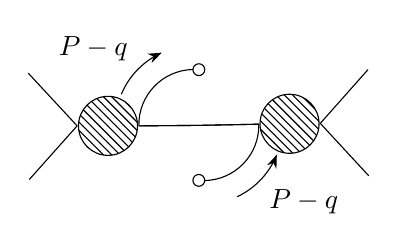
\begin{tikzpicture}[baseline=(o1.base)]
			\begin{feynman}
				\diagram[small,horizontal=o1 to o3]{
				p1 -- o1 --[draw=none] o3 -- o35 -- o4 --[draw=none] o6 -- p3;
				p2 -- o1 --[draw=none] o3 -- o35 -- o4 --[draw=none] o6 -- p4;
				};
				\node[empty dot] at ($(o3)!0.5!(o4)+(0,20pt)$) (ps1);
				\node[empty dot] at ($(o3)!0.5!(o4)+(0,-20pt)$) (ps2);
				\diagram*{
				(o3) --[quarter left,momentum={[arrow shorten=0.25]\(P-q\)}] (ps1);
				(ps2) --[quarter right,momentum'={[arrow shorten=0.25]\(P-q\)}] (o4);
				};
				\node[blob] at ($(o1)!0.5!(o3)$) (o2);
				\node[blob] at ($(o4)!0.5!(o6)$) (o5);
			\end{feynman}
		\end{tikzpicture}                                                                                                                        \\& =\mel{34}{\psi^\dagger\left(-\frac{\vb{r}}{2}\right)\psi\left(\frac{\vb{r}}{2}\right)}{12}                                                                    \\
		  & =(i\calA)^2\int\frac{\dd^4q}{(2\pi)^4}\frac{i}{q^0-\frac{\vb{q}^2}{2m}+i\epsilon}\frac{i}{\bqty{E-q^0-\frac{\vb{q}^2}{2m}+i\epsilon}^2}e^{i\vb{q}\cdot\vb{r}} \\
		  & =\calA^2\int\frac{\dd^3\vb{q}}{(2\pi)^3}\frac{m^2e^{i\vb{q}\cdot\vb{r}}}{\pqty{\vb{q}^2-p^2-i\epsilon}^2}                                                     \\
		  & =\frac{i m^2\calA^2 e^{i p r}}{8 \pi  p}
	\end{align}


\end{frame}
\begin{frame}
	\frametitle{2-pt correlator: r.h.s. (1)}

	For simplicity, we drop the external lines and focus on the internal subgraph. Consider Figure~2(b):
	\begin{flalign}
		& 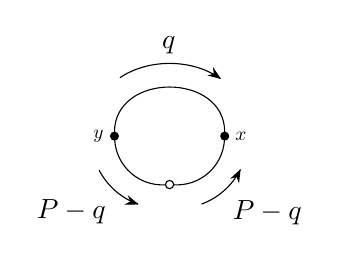
\begin{tikzpicture}[transform shape,scale=0.7,baseline=(o3.base)]
			\begin{feynman}
				\diagram[small,horizontal=o3 to o4,layered layout]{
				o3[dot,label=180:\(y\)] --[draw=none] o35 --[draw=none] o4[dot,label=0:\(x\)];
				};
				\vertex at ($(o3)!0.5!(o4)+(0,25pt)$) (ps1);
				\node[empty dot] at ($(o3)!0.5!(o4)+(0,-25pt)$) (ps2);
				\diagram*{
				(o3) --[half left,looseness=1.4,momentum={[arrow shorten=0.25]\(q\)}] (o4);
				(o3) --[quarter right,momentum'={[arrow shorten=0.25]\(P-q\)}] (ps2);
				(ps2) --[quarter right,momentum'={[arrow shorten=0.25]\(P-q\)}] (o4);
				};
			\end{feynman}
		\end{tikzpicture}=\mel{34}{\psi^\dagger\psi\left(0\right)}{12}_{amp}&&
	\end{flalign}
	\only<1>{
		\begin{align*}
			  & =\int\dd^4x\int\dd^4y\int\mm{l_1}\mm{l_2}\mm{q}e^{iP\cdot y}e^{-iP\cdot x}e^{-il_1\cdot y}e^{il_2\cdot x}e^{iq\cdot (x-y)}\tilde D(l_1)\tilde D(l_2)\tilde D(q) \\
			  & =\int\mm{q}\tilde D(P-q)\tilde D(P-q)\tilde D(q)                                                                                                                \\
			  & =-\int\mme{q}\frac{m^2}{\pqty{\vb{q}^2-p^2-i\epsilon}^2}    =-\frac{im^2}{8\pi p}
		\end{align*}
		where $\tilde D$ marks momentum space propagator and two external vertexes give an $(i\calA)^2$ factor.
	}

	\only<2>{
		The total contribution is
		\begin{align}
			\frac{im^2\calA^2}{8\pi p},
		\end{align}
		the first order Fourier expansion of the l.h.s.. The Wilson coefficient of this order is $1$.
	}
\end{frame}

\begin{frame}
	\frametitle{2-pt correlator: r.h.s. (2)}

	Figure~2(c) gives
	\begin{align}
		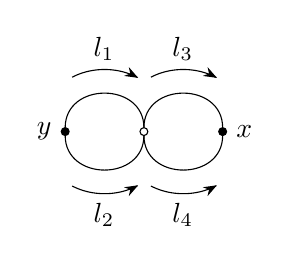
\begin{tikzpicture}[baseline=(o3.base)]
			\begin{feynman}
				\diagram[small,horizontal=o3 to o4,layered layout]{
				o3[dot,label=180:\(y\)] --[half left,momentum={[arrow shorten=0.3]\(l_1\)}] o35[empty dot] --[half left,momentum={[arrow shorten=0.3]\(l_3\)}] o4[dot,label=0:\(x\)];
				o3 --[half right,momentum'={[arrow shorten=0.3]\(l_2\)}] o35 --[half right,momentum'={[arrow shorten=0.3]\(l_4\)}] o4;
				};
			\end{feynman}
		\end{tikzpicture} & =\mel{34}{\psi^\dagger\psi^\dagger\psi\psi\left(0\right)}{12}_{amp}
	\end{align}
	which becomes
	\begin{align}
		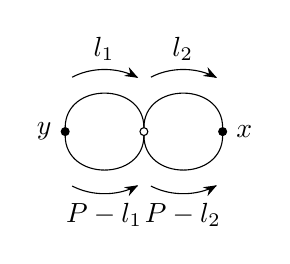
\begin{tikzpicture}[baseline=(o3.base)]
			\begin{feynman}
				\diagram[small,horizontal=o3 to o4,layered layout]{
				o3[dot,label=180:\(y\)] --[half left,momentum={[arrow shorten=0.3]\(l_1\)}] o35[empty dot] --[half left,momentum={[arrow shorten=0.3]\(l_2\)}] o4[dot,label=0:\(x\)];
				o3 --[half right,momentum'={[arrow shorten=0.3]\(P-l_1\)}] o35 --[half right,momentum'={[arrow shorten=0.3]\(P-l_2\)}] o4;
				};
			\end{feynman}
		\end{tikzpicture} & =\int\mm{l_1}\mm{l_2}\tilde D(l_1)\tilde D(P-l_1)\tilde D(l_2)\tilde D(P-l_2)                                       \\
		                           & =-\int\mme{l_1}\mme{l_2}\frac{m^2}{\left(\vb{l_1}^2-p^2-i \epsilon \right) \left(\vb{l_2}^2-p^2-i \epsilon \right)} \\
		                           & =-\mathcal{I}^2
	\end{align}

\end{frame}


\begin{frame}
	\frametitle{2-pt correlator: r.h.s. (2)}

	There're four diagrams in total:
	\begin{align}
		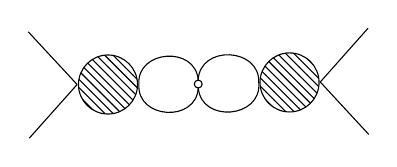
\begin{tikzpicture}[baseline=(o1.base)]
			\begin{feynman}
				\diagram[small,horizontal=o1 to o3]{
				p1 -- o1 --[draw=none] o3 --[draw=none] o35[empty dot] --[draw=none] o4 --[draw=none] o6 -- p3;
				p2 -- o1 --[draw=none] o3 --[draw=none] o35 --[draw=none] o4 --[draw=none] o6 -- p4;
				};
				\diagram*{
				(o3) --[half left] (o35) --[half left] (o4);
				(o3) --[half right] (o35) --[half right] (o4);
				};
				\node[blob] at ($(o1)!0.5!(o3)$) (o2);
				\node[blob] at ($(o4)!0.5!(o6)$) (o5);
			\end{feynman}
		\end{tikzpicture} & =\calA^2\mathcal{I}^2 \\
		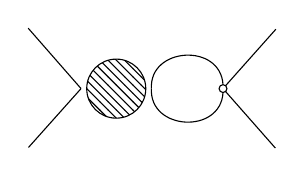
\begin{tikzpicture}[baseline=(o1.base)]
			\begin{feynman}
				\diagram[small,horizontal=o1 to o35]{
				p1 -- o1 --[draw=none] o3 --[draw=none] o35[empty dot] -- p3;
				p2 -- o1 --[draw=none] o3 --[draw=none] o35 -- p4;
				};
				\diagram*{
				(o3) --[half left] (o35);
				(o3) --[half right] (o35);
				};
				\node[blob] at ($(o1)!0.5!(o3)$) (o2);
			\end{feynman}
		\end{tikzpicture} & =\calA\mathcal{I}     \\
		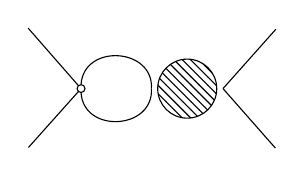
\begin{tikzpicture}[baseline=(o35.base)]
			\begin{feynman}
				\diagram[small,horizontal=o35 to o6]{
				p1 -- o35[empty dot] --[draw=none] o4 --[draw=none] o6 -- p3;
				p2 -- o35 --[draw=none] o4 --[draw=none] o6 -- p4;
				};
				\diagram*{
				(o35) --[half left] (o4);
				(o35) --[half right] (o4);
				};
				\node[blob] at ($(o4)!0.5!(o6)$) (o5);
			\end{feynman}
		\end{tikzpicture} & =\calA\mathcal{I}     \\
		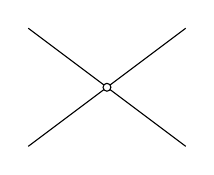
\begin{tikzpicture}[baseline=(o3.base)]
			\begin{feynman}
				\diagram[small,layered layout,horizontal=p1 to p3]{
					p1 -- o3[empty dot] -- p3;
					p2 -- o3 -- p4;
				};
			\end{feynman}
		\end{tikzpicture} & =1
	\end{align}
	We have	in total
	\begin{align}
		\expval{\psi^\dagger_1\psi^\dagger_2\psi_1\psi_2^{(\Lambda)}(0)}_{\pm\vb{p}}=(\calA\mathcal{I}+1)^2
	\end{align}

\end{frame}

\begin{frame}
	\frametitle{2-pt correlator: r.h.s. (2)}

	Plug in
	\begin{align}
		\mathcal{I}=-\frac{m}{ig(\Lambda)}-\frac{1}{\calA}
	\end{align}
	we have
	\begin{align}
		\expval{\psi^\dagger_1\psi^\dagger_2\psi_1\psi_2^{(\Lambda)}(0)}_{\pm\vb{p}}=m^2g^{-2}(\Lambda)\calA^2
		\label{2c}
	\end{align}
	The Wilson coefficient must be
	\begin{align}
		-\frac{r}{8\pi}g^2(\Lambda)
	\end{align}
	We have proven the OPE relation.


\end{frame}

\begin{frame}
	\frametitle{Momentum tail and contact}

	Let's recall some previous results:
	$$C\equiv\int\dd^3R\expval{g^2\psi^\dagger_1\psi^\dagger_2\psi_1\psi_2(R)}$$
	$$\rho_{\sigma}(\boldsymbol{k})=\int d^{3} R \int d^{3} r e^{i \boldsymbol{k} \cdot \boldsymbol{r}}\left\langle\psi_{\sigma}^{\dagger}\left(\boldsymbol{R}-\frac{1}{2} \boldsymbol{r}\right) \psi_{\sigma}\left(\boldsymbol{R}+\frac{1}{2} \boldsymbol{r}\right)\right\rangle$$
	$$\psi_{\sigma}^{\dagger}\left(\boldsymbol{R}-\frac{1}{2} \boldsymbol{r}\right) \psi_{\sigma}\left(\boldsymbol{R}+\frac{1}{2} \boldsymbol{r}\right) =1\times\psi_{\sigma}^{\dagger} \psi_{\sigma}(\mathbf{R})-\frac{g^{2}(\Lambda) r} {8 \pi}\times\psi_{1}^{\dagger} \psi_{2}^{\dagger} \psi_{1} \psi_{2}^{(\Lambda)}(\mathbf{R})+\cdots$$

	Put them together (the 1st term in OPE is 0 in large-$k$ limit):
	\begin{align}
		\rho_{\sigma}(\boldsymbol{k})\xlongequal{k\to\infty}\frac{C}{k^4}+\cdots
	\end{align}
	Note that the 3-dimensional Fourier transform of $\frac{r}{8\pi}$ is exactly $1/k^4$.

\end{frame}

\section{Applications of the Contact}
\begin{frame}
	\frametitle{Energy relation}

	According to the Hamiltonian:
	\begin{align}
		\mathcal{H} = \left(\sum_{\sigma} \frac {1} {2 m} \nabla \psi_{\sigma}^{\dagger} \cdot \nabla \psi_{\sigma}^{(\Lambda)} - \frac {\Lambda} {2 \pi^{2} m} g^{2}(\Lambda) \psi_{1}^{\dagger} \psi_{2}^{\dagger} \psi_{1} \psi_{2}\right){+ \frac {1} {4 \pi m a} g^{2}(\Lambda) \psi_{1}^{\dagger} \psi_{2}^{\dagger} \psi_{1} \psi_{2} + \mathcal{V}}
	\end{align}
	where the matrix elements of those three operators are finite. The $\nabla \psi_{\sigma}^{\dagger} \cdot \nabla \psi_{\sigma}^{(\Lambda)}$ part gives a linear divergence $2\times\frac{\Lambda  m\calA^2}{4 \pi ^2}$ for two spin states in total while the other one gives $-\frac{\Lambda m\calA^2}{2\pi^2}$, we can see that the linear divergence is cancelled. Integrating over positions, we obtain
	\begin{align}
		  &
		\begin{aligned}
			\int\dd^3R\expval{\nabla \psi_{\sigma}^{\dagger} \cdot \nabla \psi_{\sigma}} & =\int\dd^3R\dd^3r\delta^{(3)}(\vb{r})\expval{\nabla \psi_{\sigma}^{\dagger}(\vb{R-\frac{r}{2}}) \cdot \nabla \psi_{\sigma}(\vb{R+\frac{r}{2}})} \\& =\int\mme{k}k^2\rho_\sigma(k)
		\end{aligned} \\
		  & \frac {1} {4 \pi m a} \int\dd^3R \expval{g^{2}\psi_{1}^{\dagger} \psi_{2}^{\dagger} \psi_{1} \psi_{2}}=\frac {1} {4 \pi m a}C
	\end{align}


\end{frame}
\begin{frame}
	\frametitle{Energy relation}

	Also notice
	\begin{align}
		\int^\Lambda\mme{k}\frac{1}{\vb{k}^2}=\frac{\Lambda}{2\pi^2}
	\end{align}
	we have
	\begin{align}
		\int\dd^3R\frac {\Lambda} {2 \pi^{2} m} \expval{g^{2} \psi_{1}^{\dagger} \psi_{2}^{\dagger} \psi_{1} \psi_{2}}=\sum_\sigma\int\mme{k}\frac{k^2}{2m}\frac{C}{\vb{k}^4}
	\end{align}
	we achieve
	\begin{align}
		E = \sum_{\sigma} \int \frac {d^{3} k} {(2 \pi)^{3}} \frac {k^{2}} {2 m} \left(\rho_{\sigma} (k) - \frac {C} {k^{4}}\right) + \frac {C} {4 \pi m a}+ \int d^{3} R \langle V \rangle
	\end{align}

\end{frame}

\begin{frame}
	\frametitle{Adiabatic relation}

	Using F-H theorem
	\begin{align}
		\dd E / \dd a = \int \dd^{3} R \langle \partial \mathcal{H} / \partial a \rangle
	\end{align}
	it's straightforward that
	\begin{align}
		\partial \mathcal{H} / \partial a = g^{2} \psi_{1}^{\dagger} \psi_{2}^{\dagger} \psi_{1} \psi_{2} / (4 \pi m a^{2})
	\end{align}
	We then have
	\begin{align}
		\frac {\dd E} {\dd (1 / a)} = - \frac {1} {4 \pi m} C
	\end{align}

\end{frame}
\begin{frame}
	\frametitle{Virial theorem}

	Given a harmonic trapping potential:
	\begin{align}
		V(\vb{R})=\frac{m}{2}\omega^2R^2
	\end{align}
	Dimensional analysis requires
	\begin{align}
		\bqty{\omega\pdv{\omega}-\frac{1}{2}a\pdv{a}}\int\dd^3R\expval{\mathcal{H}}=\int\dd^3R\expval{\mathcal{H}}
	\end{align}
	Together with F-H theorem
	\begin{align}
		  & \frac{a}{2}\pdv{a}\int\dd^3R\expval{\mathcal{H}}=\frac{C}{8\pi m a}                                                   \\
		  & \pdv{\omega}\int\dd^3R\expval{\mathcal{H}}=\pdv{\omega}\int\dd^3R\expval{\mathcal{V}}=2\int\dd^3R\expval{\mathcal{V}}
	\end{align}
	\begin{align}
		E=2 \int d^{3} R\langle\mathcal{V}\rangle-C /(8 \pi m a)
	\end{align}

\end{frame}

\begin{frame}
	\frametitle{Number density operator of fermion pairs}

	We have number density operator for fermion pairs
	\begin{align}
		\psi_1^\dagger\psi_1(\vb{R}-\frac{1}{2}\vb{r})\psi_2^\dagger\psi_2(\vb{R}+\frac{1}{2}\vb{r})
	\end{align}
	and the diagram is
	\begin{align*}
		  & 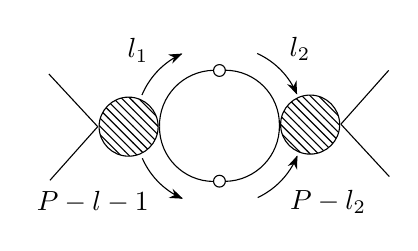
\begin{tikzpicture}[baseline=(o1.base)]
			\begin{feynman}
				\diagram[small,horizontal=o1 to o3]{
				p1 -- o1 --[draw=none] o3 --[draw=none] o35 --[draw=none] o4 --[draw=none] o6 -- p3;
				p2 -- o1 --[draw=none] o3 --[draw=none] o35 --[draw=none] o4 --[draw=none] o6 -- p4;
				};
				\node[empty dot] at ($(o3)!0.5!(o4)+(0,20pt)$) (ps1);
				\node[empty dot] at ($(o3)!0.5!(o4)+(0,-20pt)$) (ps2);
				\diagram*{
				(o3) --[quarter left,momentum={[arrow shorten=0.25]\(l_1\)}] (ps1);
				(ps1) --[quarter left,momentum={[arrow shorten=0.25]\(l_2\)}] (o4);
				(o3) --[quarter right,momentum'={[arrow shorten=0.25]\(P-l-1\)}] (ps2);
				(ps2) --[quarter right,momentum'={[arrow shorten=0.25]\(P-l_2\)}] (o4);
				};
				\node[blob] at ($(o1)!0.5!(o3)$) (o2);
				\node[blob] at ($(o4)!0.5!(o6)$) (o5);
			\end{feynman}
		\end{tikzpicture}                                                                                                                                                                                                                                \\
		  & =(i\calA)^2\int\mm{l_1}\mm{l_2}\frac{i}{l_1^0-\frac{\vb{l_1}^2}{2m}+i\epsilon}\frac{i}{{E-l_1^0-\frac{\vb{l_1}^2}{2m}+i\epsilon}}\frac{i}{l_2^0-\frac{\vb{l_2}^2}{2m}+i\epsilon}\frac{ie^{i\vb{q}\cdot\vb{r}}}{{E-l_2^0-\frac{\vb{l_2}^2}{2m}+i\epsilon}} \\
		  & =\frac{\calA^2m^2 }{16 \pi ^2 r^2}e^{2 i p r}
	\end{align*}
	Compare with the result of Figure~2(c) \eqref{2c} we have
	\begin{align}
		\psi_{1}^{\dagger} \psi_{1}\left(\boldsymbol{R}-\frac{1}{2} \boldsymbol{r}\right) \psi_{2}^{\dagger} \psi_{2}\left(\boldsymbol{R}+\frac{1}{2} \boldsymbol{r}\right) \rightarrow \frac{1}{16 \pi^{2} r^{2}} g^{2} \psi_{1}^{\dagger} \psi_{2}^{\dagger} \psi_{1} \psi_{2}(\boldsymbol{R})
	\end{align}

\end{frame}
\begin{frame}
	\frametitle{Contact?}

	Define $N_{\mathrm{pair}}(\boldsymbol{R}, s)$ to describe the number of fermion pairs within a sphere of radius $s$
	$$N_{\mathrm{pair}}(\boldsymbol{R}, s)\equiv \int_{\abs{\vb{r}}<s}\dd^3\vb{r}\psi_{1}^{\dagger} \psi_{1}\left(\boldsymbol{R}-\frac{1}{2} \boldsymbol{r}\right) \psi_{2}^{\dagger} \psi_{2}\left(\boldsymbol{R}+\frac{1}{2} \boldsymbol{r}\right)$$

	In the absence of interactions, $\left\langle N_{\text {pair }}(\boldsymbol{R}, s)\right\rangle$ scales as $s^{3}$ as $s \rightarrow 0$.

	In the case of a large scattering length $\left\langle N_{\text {pair }}(\boldsymbol{R}, s)\right\rangle$ scales as $s^{1}$. We can interpret the contact density operator $g^{2} \psi_{1}^{\dagger} \psi_{2}^{\dagger} \psi_{1} \psi_{2}$ as the limit as $s \rightarrow 0$ of $(4 \pi / s) N_{\text {pair }}(R, s)$.

	Consider inelastic scattering into other spin states that has much lower energy. The effect on a state with definite energy $E$ is to change its time-dependence from $\exp (-i E t)$ to $\exp (-i(E-i \Gamma / 2) t ) $. The probability
	in that state decreases with time at the rate $\Gamma $. The adiabatic relation can be used to derive an expression for $\Gamma$ to leading order in the imaginary part of $a$
	\[
		\Gamma \approx \frac{(-\operatorname{Im} a)}{2 \pi m|a|^{2}} C
	\]
	Thus $C$ determines the rate at which low-energy fermions are depleted by inelastic collisions.

\end{frame}


% \section*{END}

% \begin{frame}
% 	\begin{center}
% 		\Huge 
% 		\usebeamercolor[bg]{frametitle}
% 		\emph{Thanks for your attention!}
% 	\end{center}
% \end{frame}

\appendix
\begin{frame}[standout]
	\Huge Questions?
\end{frame}
\begin{frame}
	\vfill
	\centering
	\begin{beamercolorbox}[sep=8pt,center,shadow=true,rounded=true]{title}
		\usebeamerfont{title}Backup\par%
	\end{beamercolorbox}
	\vfill
\end{frame}

\begin{frame}
	\frametitle{PDS scheme~\parencite{Kaplan:1998tg}}

	We start with the one loop bubble in $d\to3$ dimension, for latter convenience we rescale the usual $\mu$ by $1/2$
	\begin{align}
		\mathcal{I}=-i\pqty{\frac{\mu}{2}}^{3-d}\int\mmd[d]{\vb{l}}\frac{m}{\vb{l}^2-p^2}=-i\frac{ \pi ^{1-\frac{d}{2}} m \mu ^{3-d} \left(-\frac{1}{p^2}\right)^{1-\frac{d}{2}} \csc \left(\frac{\pi  d}{2}\right)}{\Gamma \left(\frac{d}{2}\right)}
	\end{align}
	For MS scheme, we only subtract poles at $d=3$. For PDS scheme, we also subtract poles at $d=2$. The counterterm is 
	\begin{align}
		\delta \mathcal{I}=\frac{-i\mu m }{4 \pi(d-2)}
	\end{align}
	Now we add $\delta \mathcal{I}$ to $\mathcal{I}$, then expand the expression in $d=3$: 
	\begin{align*}
		\mathcal{I}+\delta \mathcal{I}=\frac{-im(\mu+i p)}{4 \pi}
	\end{align*}
	The total amplitude is
	\begin{align}
		i\calA_{\mathrm{PDS}} & =\frac{-1}{\mathcal{I}+\frac{m}{ig(\mu)}}=\frac{-1}{\frac{-im(\mu+i p)}{4 \pi}+\frac{m}{ig(\mu)}}
	\end{align}
\end{frame}
\begin{frame}
	\frametitle{PDS scheme}

	With a little algebra
	\begin{align*}
		i\calA_{\mathrm{PDS}}=\frac{-1}{\frac{-im(\mu+i p)}{4 \pi}+\frac{m}{ig(\mu)}}=\frac{4i\pi/m}{-\mu-\frac{4\pi}{ig(\mu)}-ip}
	\end{align*}
	We have
	\begin{align}
		g(\mu)=\frac{-4\pi i}{1/a-\mu}
	\end{align}

	In hard cutoff scheme, by simple power-counting, the tree diagram is leading. But that's not true, because there're cancellations between orders. In the end, one needs to resum all orders. 

	In PDS scheme, we can see all orders are of the same magnitude, thus the need for resummation is explicit. 
\end{frame}


\printbibliography

% \bibliography{../Bib}
% \bibliographystyle{apalike}

\end{document}